\subsection{Airframe}
In this year's mission, the aircraft is required to cover more than 10km in less than 10 min. Furthermore, the aircraft should perform one 'mission lap' at high speed (just less than 60kts). Thus multirotor concepts are much less suited than in previous competition years, as their inferior aerodynamic efficiency would require large batteries and thus reduce the carried payload. Hence it was decided to employ a fixed wing design. Although other participants in the UAS challenge have successfully made use of flying wing concepts in previous years, this concept was deemed less suitable as it is less modular than a traditional aircraft with an empennage, so that the tail components of the aircraft are individually replacable in case of a crash. The same rationale was applied to the selection of the tail configuration. The H-tail allows for individual replacing of the horizontal and vertical stabilisers. This would not be possible with e.g. a V-tail. The modular design philosophy was applied to other parts of the UAV as well, for instance the servos are individually replacable.

The UAV features high aspect ratio wings (AR=8.64) to reduce drag. The wings are manufactured from hot wire cut foam and covered in fibreglass using a novel technique developed by the team. The same technique is used for the manufacturing of the tail surfaces.

The fuselage is made from fibreglass, using a CNC-machined mould. 

\subsection{Propulsion}
The UAV features a single 800W electric motor to allow for maximum speed during the mission. The propeller is of diameter 16in, to maximise propulsive efficiency. The battery has 4 cells and a capacity of 2500mAh.

\subsection{Payload release}
As payload release mechanism a commercially available unit is used, controlled by a servo. The payload bay automatically opens when the payload is released, as the weight of the payload pushes open the payload bay doors, which are held closed by little springs. This approach reduces mechanical and electronic complexity, as the payload bay door opening components are completely passive.

\subsection{Flight Control System}
The flight control system on board the UAV encompasses areas such as stability augmentation, navigation, and mission control. These tasks are performed on a completely custom 32-bit ARM-based microcontroller board, which has all required sensors and interfaces directly on it. Additionally, a Raspberry Pi 3+ single-board computer as well the corresponding Pi v2 camera is used for the tasks that require image processing and recognition. Finally, a 2.4GHz spread-spectrum transceiver is used both on the UAV and at the basestation to enable the transmission of mission-critical data. A block diagram overview of the entire system is given in Figure \ref{fig:SysBlockDiag} below.

\begin{figure}[H]
\centering
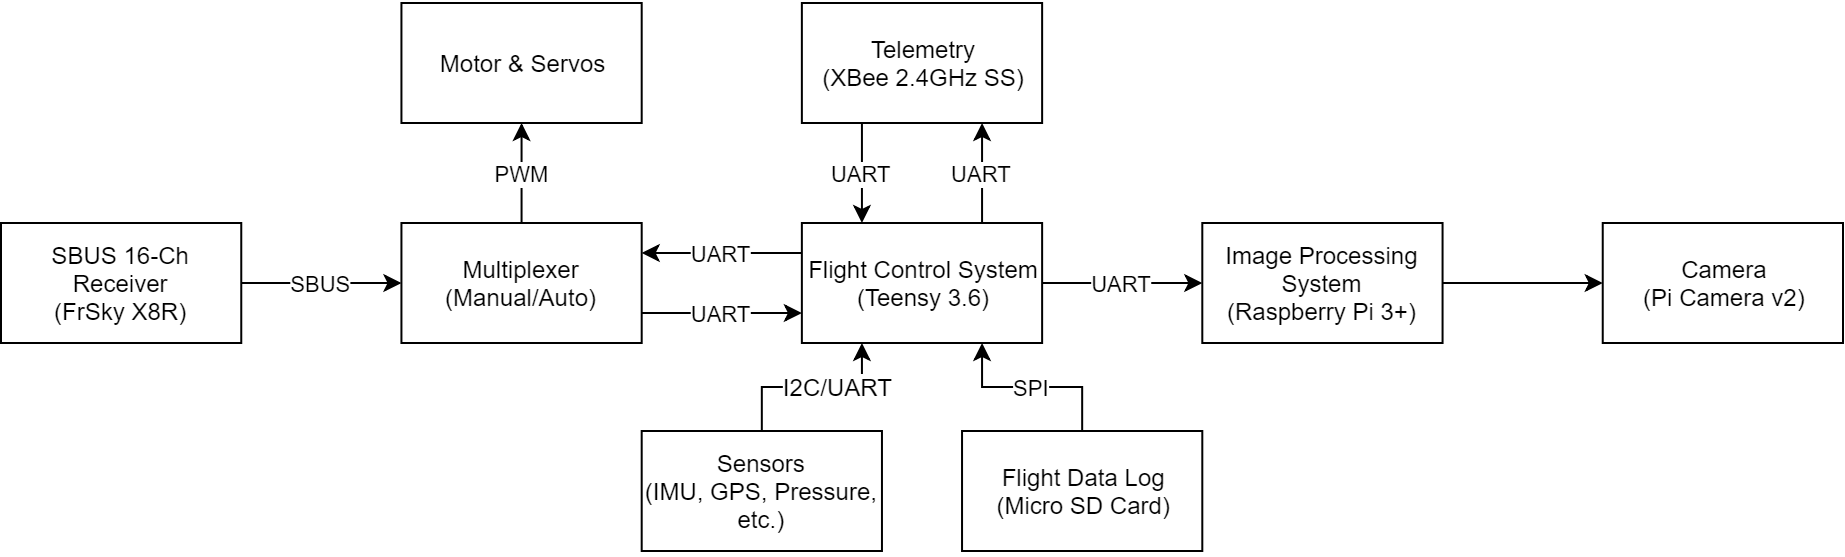
\includegraphics[scale=0.3]{figs/SysBlockDiagram.png}
\caption{System Block Diagram}
\label{fig:SysBlockDiag}
\end{figure}

\subsubsection{Stability}
Closed-loop feedback control is used for stability and provides a robust platform for the higher level autopilots on board the UAV to build on. Feedback is provided from various sensors, e.g. angle of attack, IMU, sideslip (see \textit{Sensor} section below). Dynamic states not directly measurable are estimated using an \textit{Extended Kalman Filter}. \\

The control system was designed using an $H_{\infty}$ loop-shaping approach. This state-of-the-art method of designing control systems combines the classical single-input-single-output (SISO) loop-shaping procedure of classical feedback theory with more modern state-space control, providing benefits of both worlds such as state decoupling, multi-variable feedback, and intuitive setting of closed-loop requirements. Additionally, robustness is guaranteed by giving controllers that meet certain performance specifications even when the system's dynamic model is only approximately known. \\

The UAV's dynamic model was acquired using AVL (DATCOM alternative) which estimates the aerodynamic coefficients and stability derivatives from 3D model data. These coefficients were combined with the equations of motion to give an approximate model of the system with which control design could be performed. \\

\subsubsection{Sensors}
Sensors used for feedback control, as well as higher level features such as GPS navigation, available on the UAV are: \textit{IMU, GPS, Angle of Attack, Sideslip, Camera, Airspeed (Pitot), Barometer, Temperature}.

\subsubsection{Navigation and Mission Control}
Autonomous navigation and mission control is entirely performed on the previously mentioned custom microcontroller board. The system runs as a state machine switching between discrete states as needed, for instance for take-off, reconnaissance, landing, and so forth. The navigation system utilizes the lower-level functionality of the previously described stability augmentation system to set desired roll angles, altitude, airspeed, etc.

\subsection{Image Processing}
The image processing and recognition is performed using a Raspberry Pi 3+ and a Pi v2 camera. The image recognition script is written in Python in combination with the OpenCV library. The system is running constantly, with a description of currently recognised targets being relayed to the main flight control system via a UART serial interface.

\subsection{Innovative Features}
\begin{itemize}
	\item State-of-the-art $H_{\infty}$ control system.
	\item Custom, high-speed electronic sub-systems.
	\item In-flight system identification.
	\item Novel manufacturing technique for glassing of wings.
	\item Modular mechanical design.
\end{itemize}

\subsubsection{Flight Termination System (FTS)}
See section \ref{sec:fts}.

\subsection{Three view drawing}
\vspace*{-0.4cm}
\begin{figure}[H]
	\centering
	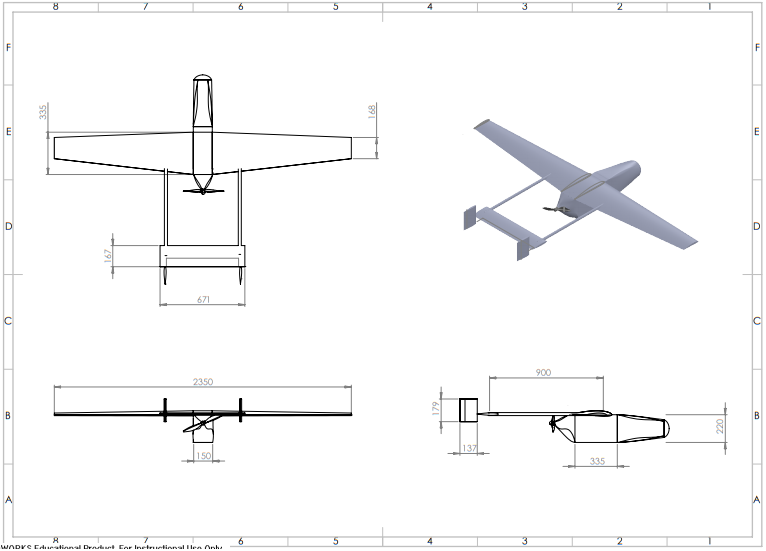
\includegraphics[width=\textwidth]{three_view_drawing}
\end{figure}
